\startchapter{Deformable Model}
\label{chapter:deformablemodel}
Interactive visualization techniques developed in the previous chapters support a \blob based modelling 
system for the incremental construction process. In a surgical simulation scenario, tissues undergo 
various levels of deformations and topological modifications. Researchers in the field studied different 
approaches to recreate the elastic behavior of tissues. The two main challenges that are reported 
continuously in this field are interactivity and fidelity of motion \cite{Meier2005}. 

Based on the foundation built so far, we create a deformable model to support the required interactions 
with surgical tools i.e., elastic deformations by pushing the tissue. 
The next chapter will address the problem associated with cutting, which is a primary operation in 
many surgical simulation scenarios. The goal is to make a comprehensive system that bridges the gap 
between modelling and simulation of tissues. 

\section{Overview}
A software pipeline is developed to support physically based simulation of deformable tissues using our 
implicit modelling framework, figure \ref{fig:systempipeline}. 

\begin{figure}[H]
  \centering
  % the following command controls the width of the embedded PS file
  % (relative to the width of the current column)
  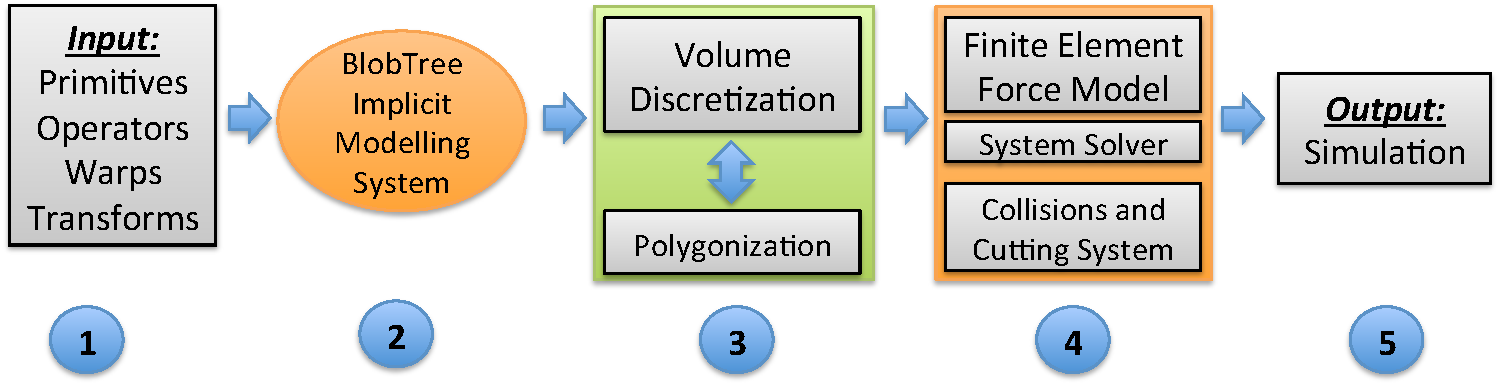
\includegraphics[width=1.0\linewidth]{figures/deformable/pipeline.pdf}
  \caption{\label{fig:systempipeline}
  {High-level system software pipeline to support deformations and cutting. }
}
\end{figure}

Stages 1 and 2 in the pipeline are associated with the modelling process which is 
already discussed in chapter \ref{chapter:background}. Stage 3 is 
associated with the polygonization algorithms that are developed in chapters \ref{chapter:cpuPoly} 
and \ref{chapter:GPUDiscretization}. Also in stage 3 is the volume discretization technique that converts 
the \blob model into a tetrahedral mesh for physical simulation, this process is discussed further in 
section \ref{sec:physicalmodel}. The material that is discussed in the current and the next chapters are associated with the 
stage 4 of the pipeline shown above. The output of the system is the simulation environment that 
facilitates deformations and cutting which is shown as the final stage. 


\section{Physical Model}
\label{sec:physicalmodel}
The deformable model has to be considered as a continuous volume in order to reproduce its elastic, 
volumetric effects. In our system, the \blob model is discretized into a tetrahedral mesh using the 
algorithm proposed by Labelle \etal \cite{Labelle2007}. This step is performed once the modelling stage is
completed and the tissue is ready for the simulation. This is a one time process and is not a bottleneck 
in our system. 

A fine-grained cell-size parameter captures the exterior part of the model while a coarser sampling is 
used to produce the internal tetrahedral cells. This approach allows us to maintain a balanced number 
of tetrahedral cells for the physics simulation. The output of this stage is called \textit{volume mesh} in 
order to differentiate it from the surface mesh which is extracted using the polygonization algorithm in 
the previous chapters. The data structure representing the tetrahedral meshes in our system is described 
in section \ref{sec:tetmeshstructure}.

%describe our finite element force model

\section{Collision and Contact with tools}
\label{sec:collisionsandcontacts}
The interactions of medical devices and the tissue model has to be accounted for to support surgical 
training scenarios. The way these contacts are handled impacts the overall behavior of the system with 
respect to the deformable tissues. Figure \ref{fig:contact}, shows the overall 
collision and contact handling.

\begin{figure}[H]
  \centering
  % the following command controls the width of the embedded PS file
  % (relative to the width of the current column)
  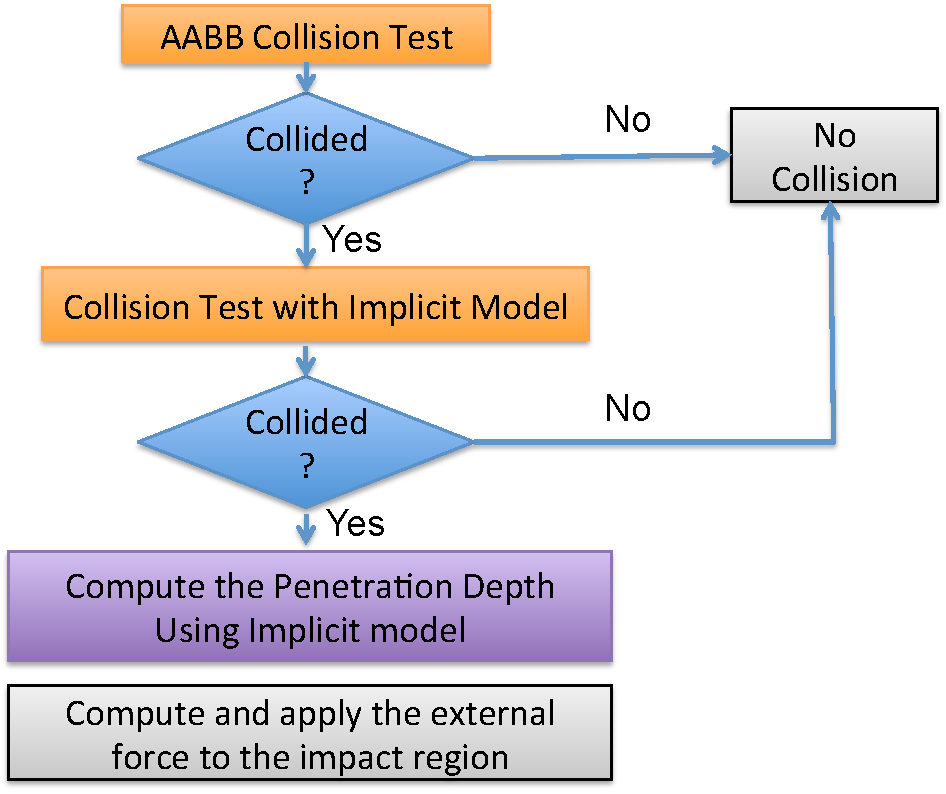
\includegraphics[width=0.8\linewidth]{figures/deformable/contact.pdf}
  \caption{\label{fig:contact}
  {To compute the external forces applied to the physical model, we exploit the trivial collision detection 
  facilities of the underlying implicit model.}
}
\end{figure}

Medical tools are modelled as simple polygonal shapes in our system. The user moves the tool freely 
and to compute the collision of the tool and the model several steps are performed in order. First, the 
axis aligned bounding box (AABB) of the tool is tested against the AABB of the model and if an 
intersection is detected the process continues further. The second collision 
test is performed by computing the field at vertices of the tool model. In case 
of our probing tool which is modelled as a cube, the field due to the vertices of the cube are computed. 
If a field at a vertex is above the \textit{iso-value}, then that vertex is inside the model and an intersection 
is detected.

To compute the distance, the inverse of the field function from equation \ref{eq:WyvillFunc} 
is used:

\begin{equation}
dist_\mathrm{wyvill}(f)= \left\{ \begin{array}{rl}
 1 &\mbox{ if $f = 0$} \\
\sqrt{ (1-f^\frac{1}{3}) } - k &\mbox{ if $0 < f \leq 1$}
 \end{array} \right.
\label{eq:InverseWyvillFunc}
\end{equation}

In equation \ref{eq:InverseWyvillFunc}, $f$ is the input field and $k$ is called the 
\textit{iso-distance} value which is the perpendicular distance from the iso-surface to the nearest skeleton 
of the model. $k$ can be computed easily by using the the $iso-value$ which is set to 0.5 in our system 
as the output of equation \ref{eq:WyvillFunc}, solving that equation for $x$ yields to the constant value of 
0.4541 for $k$. 


\begin{figure}[H]
  \centering
  % the following command controls the width of the embedded PS file
  % (relative to the width of the current column)
  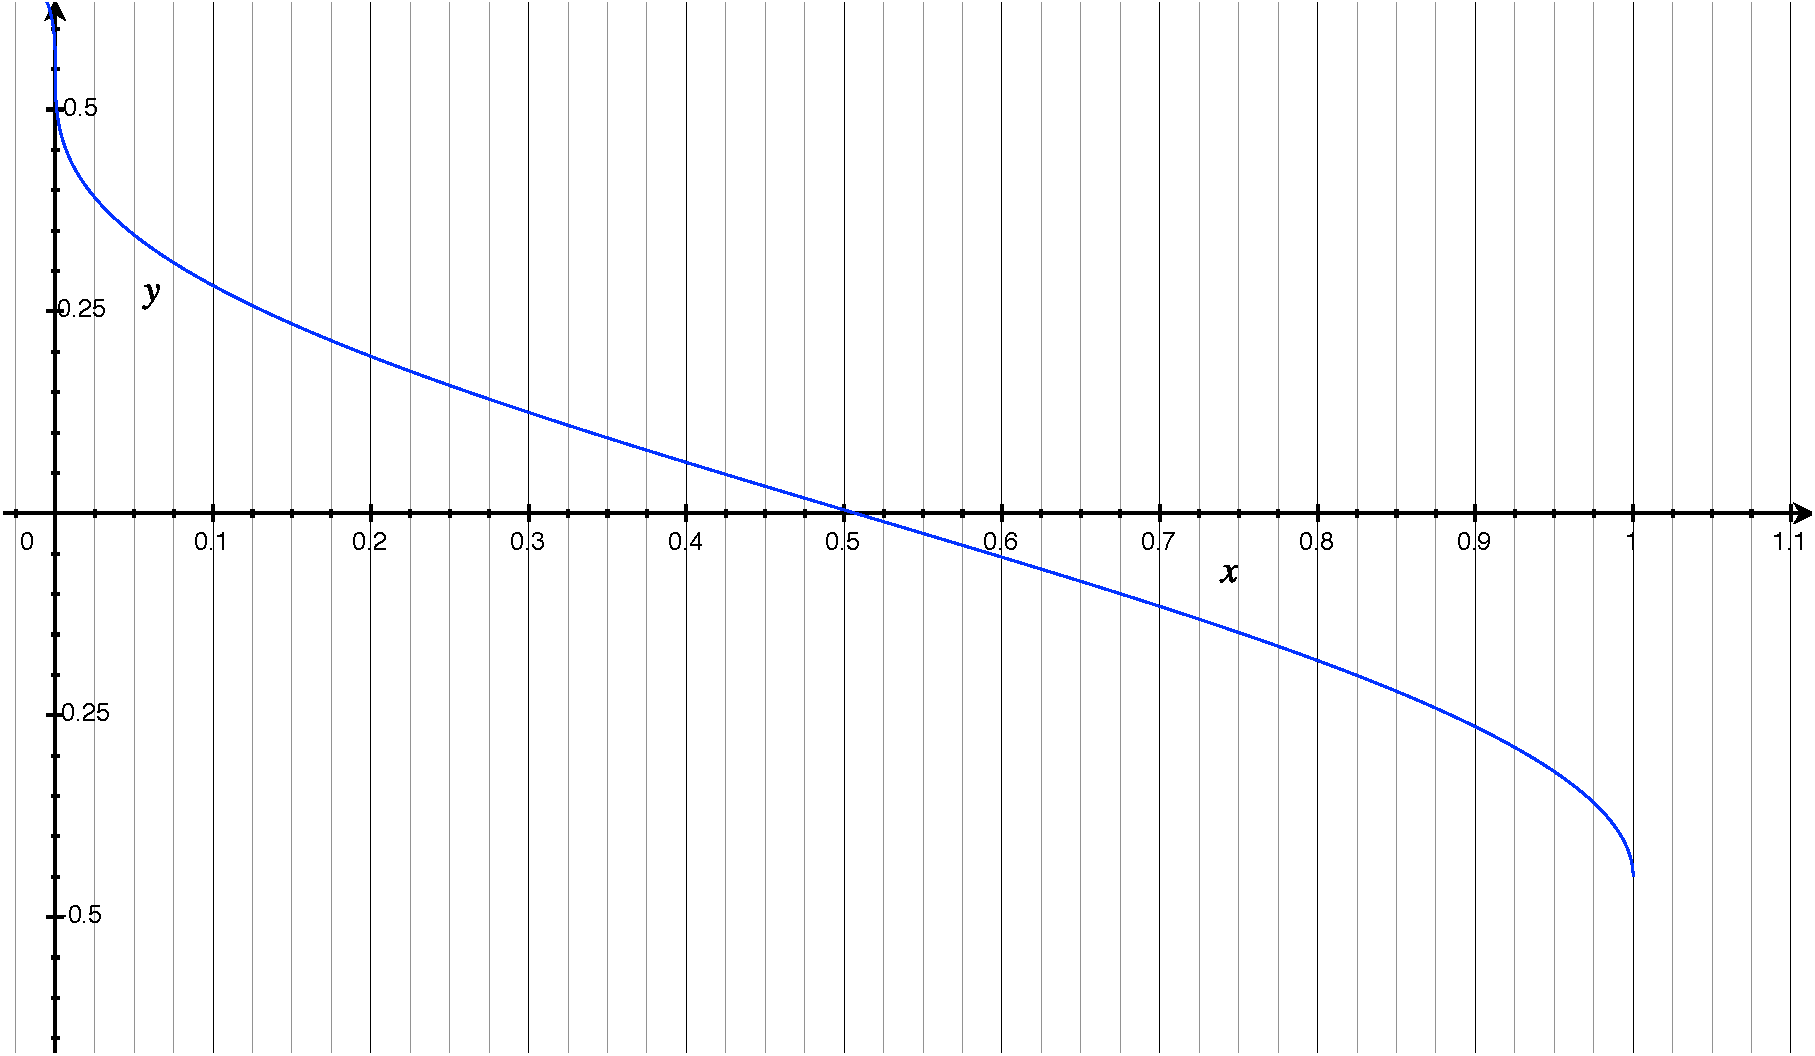
\includegraphics[width=0.8\linewidth]{figures/deformable/distancefromfield.pdf}
  \caption{\label{fig:distancefromfield}
  {Plot of equation \ref{eq:InverseWyvillFunc}. Horizontal axis is the field value which is changing from 0 to 1
 in this graph. The vertical axis is the distance to the \textit{iso-surface}.}
}
\end{figure}

Figure \ref{fig:distancefromfield}, is the plot of equation \ref{eq:InverseWyvillFunc} 
in the range $\left[0, 1\right]$ for the field value. When the field is equal to 
the \textit{iso-value}, then the associated vertex is on the surface, hence the zero distance. 
A positive value for distance is due the fact that the collision has not happened yet but the vertex 
is in close proximity of the surface, whereas negative values indicate a penetration into the model. 

In case of a collision, the penetration depths are computed for the all colliding vertices of the tool.
The interaction force is computed based on the computed penetration depths. The 
contact force is computed using the direction of the tool and the gradient of the field as shown in the 
following equation:

\begin{equation}
CF(v) = (\frac{\nabla F(v) + T} { \| \nabla F(v) + T \|}) * dist_\mathrm{wyvill}( g_\mathrm{wyvill}(v)) * 
s
\label{eq:contactforce} 
\end{equation}

The output of equation \ref{eq:contactforce} is a force vector at point $v$, $T$ is a directional vector that 
represents the tool trajectory. The direction of the final external force is adjusted using the gradient of 
the field i.e., instead of using the tool trajectory vector $T$ directly; we use the average of $T$ and the field 
gradient at $v$. This choice is made to compensate for the tangential tool trajectories that can cause 
unintended shearing at the boundary edges of the model.

$g_\mathrm{wyvill}(v)$ and $\nabla F(v)$ are the field and gradient at vertex $v$, respectively. $s$ 
is the impact factor to adjust the external force magnitude.

Using this technique, the contact forces are computed upon collisions of the tool and the model. To
apply this external force to the physical model we use a force propagating technique based on 
the volume mesh data structure described in section \ref{sec:tetmeshstructure}. 

The edge-based data structure for the tetrahedral mesh provides access to all the adjacent vertices to a 
given vertex. This functionality can provide the access to the K-ring neighborhood of a contact point to 
perform force propagation. Figure \ref{fig:kring}, shows an example of this function for a contact 
point $p$. The external force computed for $P$ is propagated to the first and second rings with 
decreasing magnitudes at each step. This technique provides a more realistic 
distribution of the collision force for the simulation of tool-model interactions.
 
 \begin{figure}[H]
  \centering
  % the following command controls the width of the embedded PS file
  % (relative to the width of the current column)
  
\includegraphics[width=7.0\linewidth]{figures/deformable/kring.pdf}
  \caption{\label{fig:kring}
  {The K-ring neighborhood of a vertex $p$ can be accessed using our tetrahedral mesh 
  data-structure. The first and second rings of vertex $p$ are shown in orange and pink here, respectively.}
}
\end{figure}


\section{Results}
In this section we present our results in simulating the behavior of several deformable models created 
using our implicit modelling framework. Table \ref{table:deformablemodels}, provides details of the 
models. The number of tetrahedral cells reported in this table are extracted using a small cellsize of 0.1. 

\begin{table}[H]
\begin{center}
\caption{\label{table:deformablemodels}
{The following deformable models are used in our experiments.}}
  \begin{tabular}{ | l | c | c | c | }
    \hline    
    name & primitives & operators & finite element cells \\ \hline \hline    
    tumor & 10 & 1 & 130K \\ \hline
    3slabs & 4 & 1 & 120K \\ \hline
    cake & 11 & 1 & 85K \\ \hline
    \hline
  \end{tabular}
\end{center}
\end{table}

Figure \ref{fig:cellsize_elements} shows the effect of cellsize parameter in the number of finite element 
cells generated for the physical mesh. As shown in this graph, increasing the step size for the volume 
discretization process, results in larger finite element cells and decreases the total count of elements.

\begin{figure}[H]
  \centering
  % the following command controls the width of the embedded PS file
  % (relative to the width of the current column)
  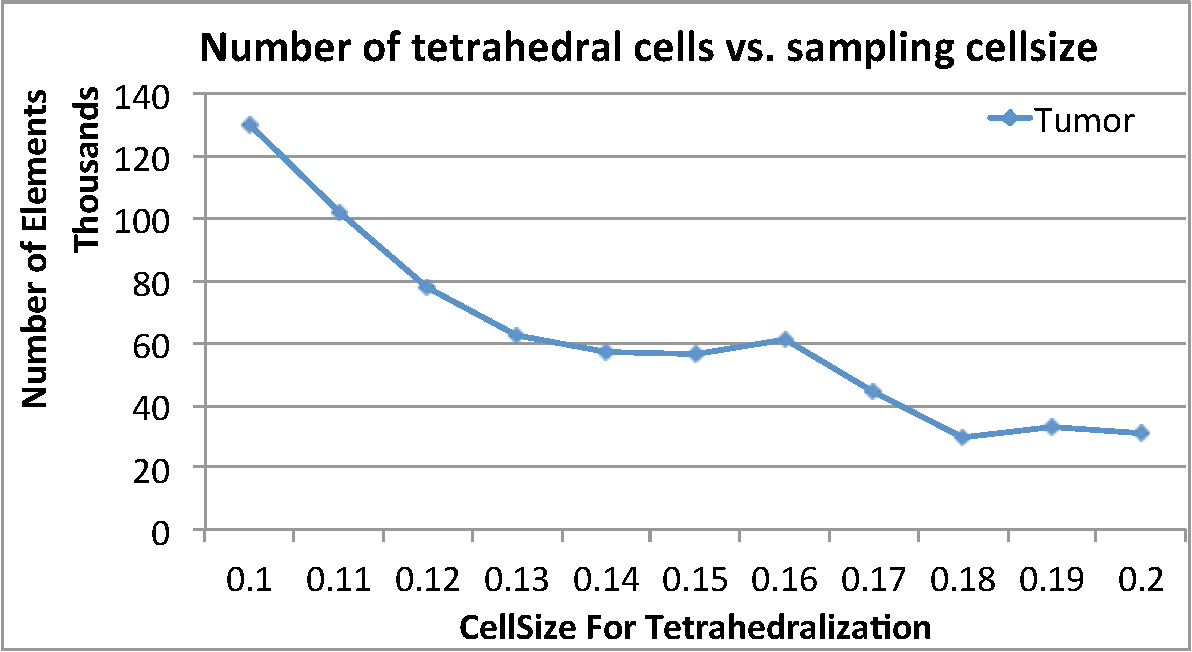
\includegraphics[width=0.8 \linewidth]{figures/deformable/cellsize_elements.pdf}
  \caption{\label{fig:cellsize_elements}
  {The effect of cellsize parameter in the total number of generated tetrahedral cells for the physics mesh.}
}
\end{figure}

Figure \ref{fig:tumor} and \ref{fig:3slabs} show the tumor and the 3slabs models when compressed with 
the probe tool, respectively. The surface mesh which is extracted with our polygonization method is 
deformed using the computed displacements for the volume mesh. The 3slabs model 
in figure \ref{fig:3slabs} is fixed to the green wall and the external forces applied by the probe tool 
barely reach the green slab. 

\begin{figure}[H]
  \centering
  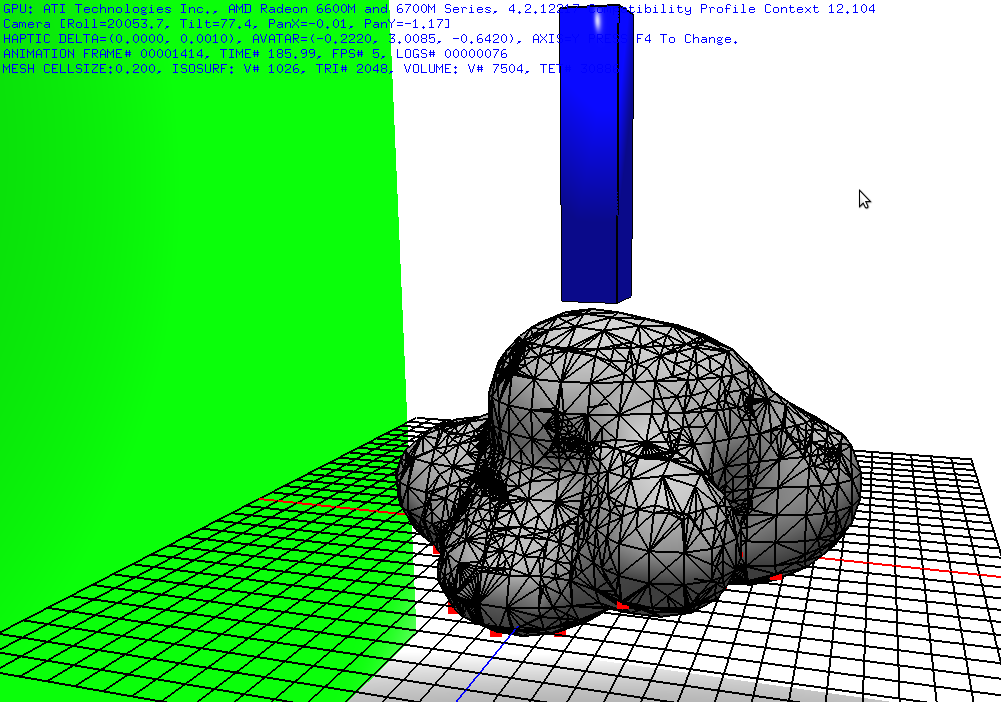
\includegraphics[width=0.30\linewidth]{figures/deformable/shots/tumor01.png}
  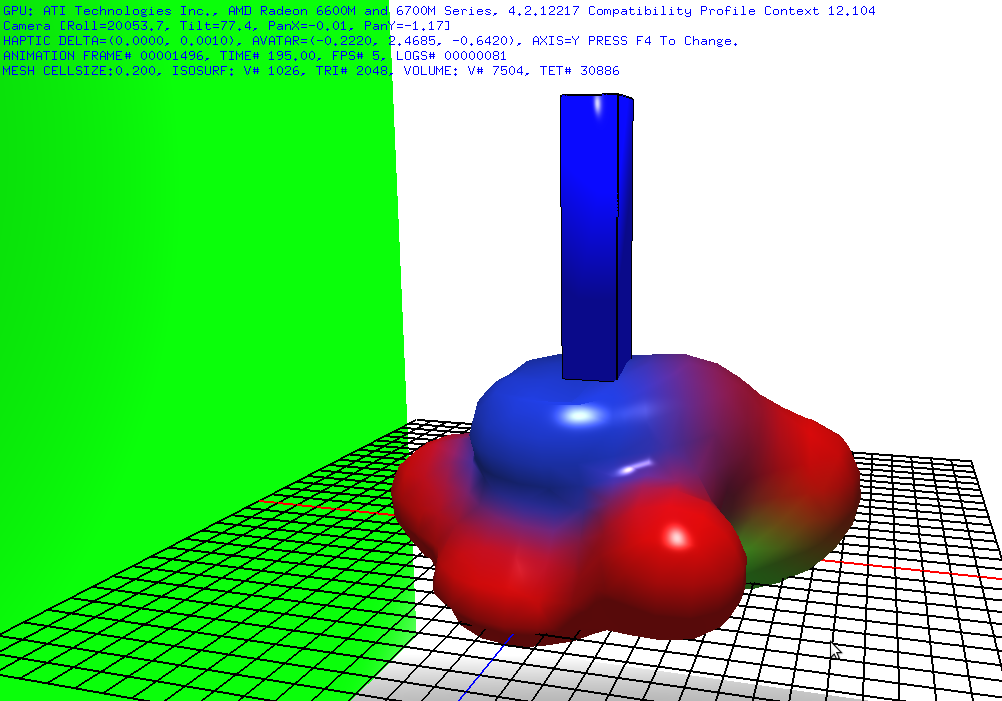
\includegraphics[width=0.30\linewidth]{figures/deformable/shots/tumor02.png}
  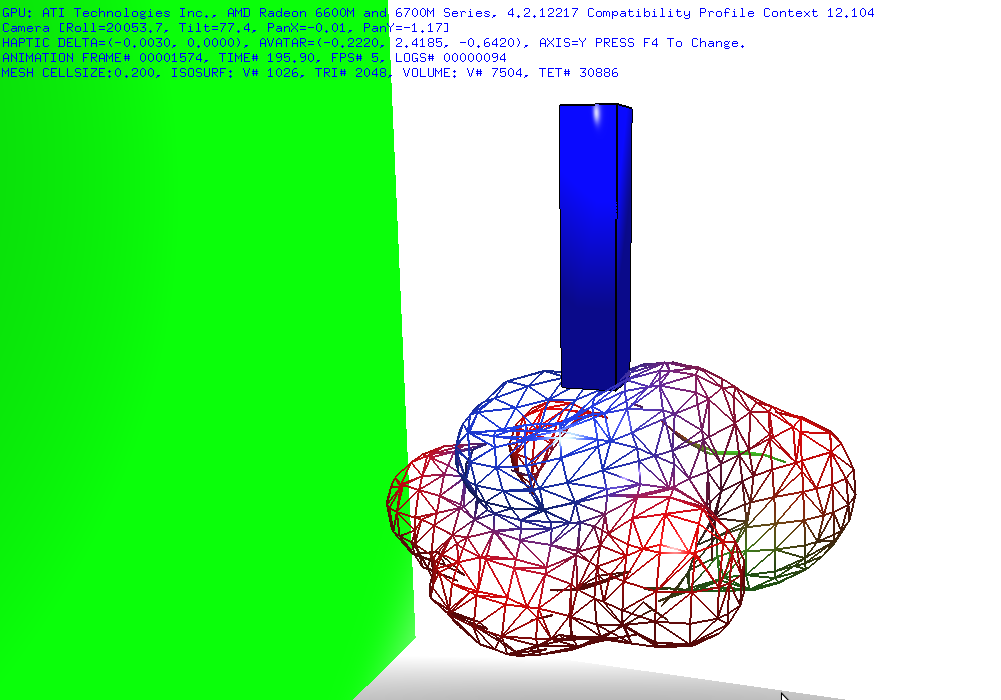
\includegraphics[width=0.30\linewidth]{figures/deformable/shots/tumor03.png}
 
  \caption{\label{fig:tumor}
  {Tumor model is pushed from the top using our probe tool. Left: The volume mesh used as physics 
  model shown in gray. Middle: Model pushed down for compression. Right: The surface mesh deformations
  are in sync with that of the volume mesh.}
}
\end{figure}

\begin{figure}[H]
  \centering
  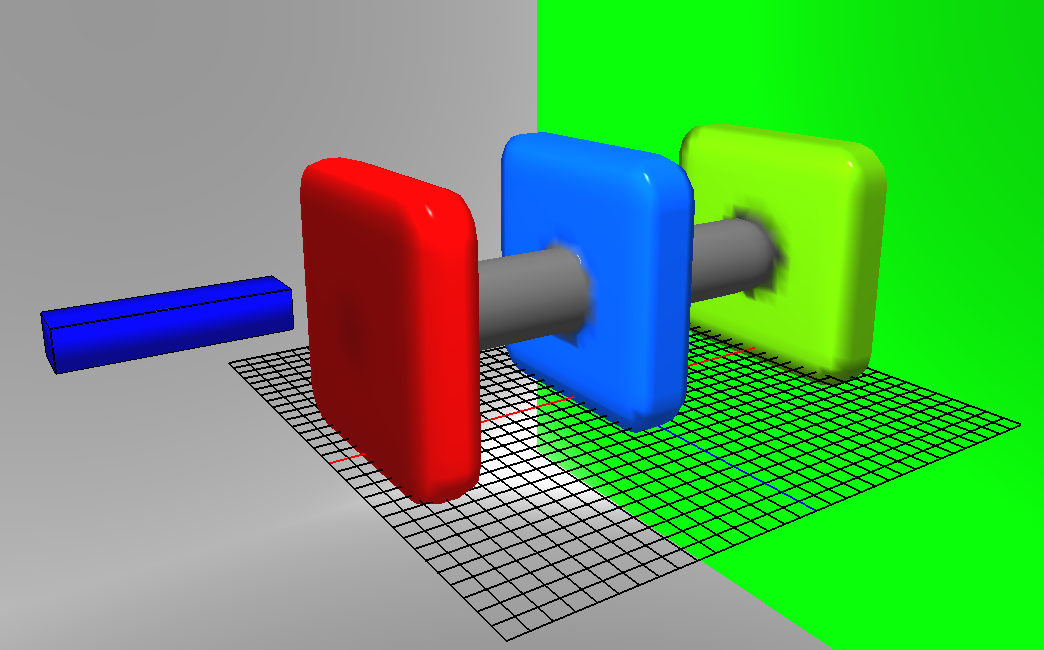
\includegraphics[width=0.30\linewidth]{figures/deformable/shots/3slabs01.png}
  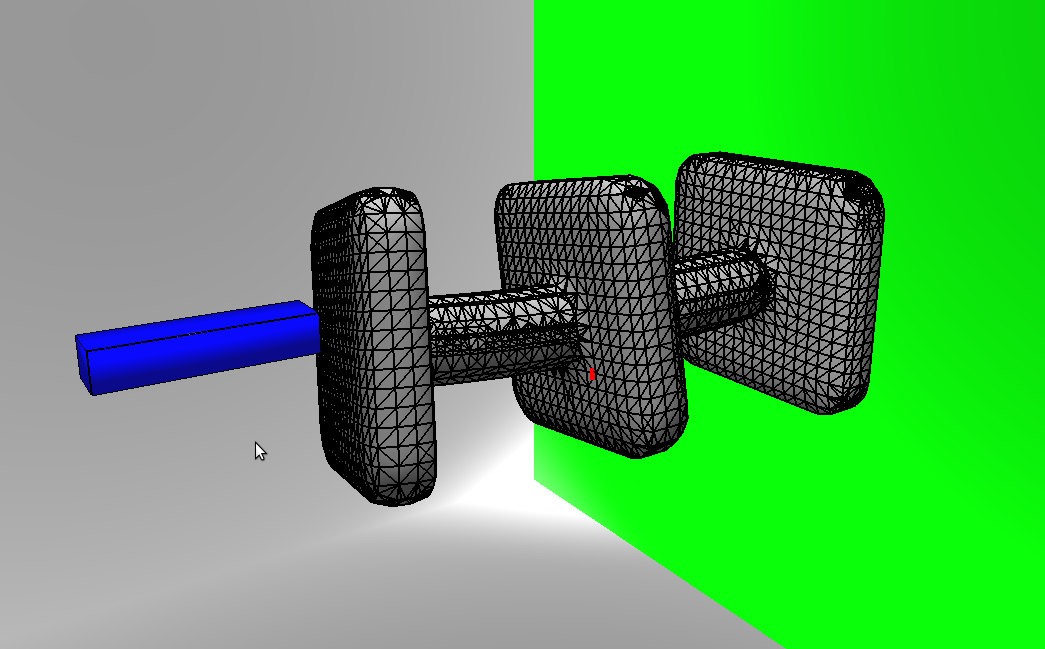
\includegraphics[width=0.30\linewidth]{figures/deformable/shots/3slabs02.png}
  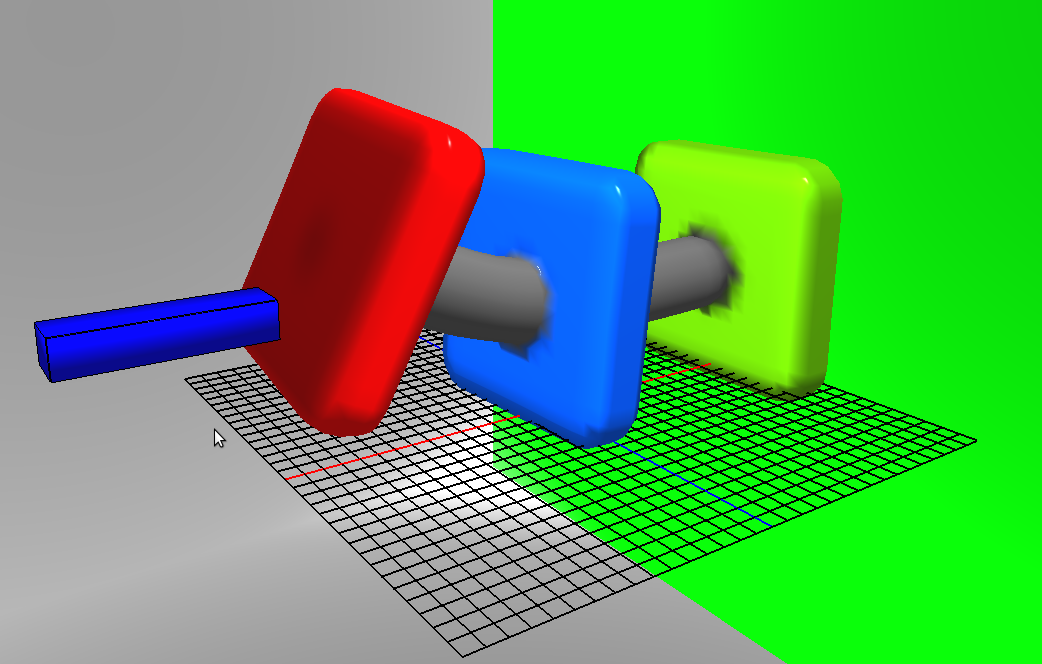
\includegraphics[width=0.30\linewidth]{figures/deformable/shots/3slabs03.png}
 
  \caption{\label{fig:3slabs}
  {The force is applied to the 3slabs model horizontally. The green slab is fixed to the wall in this experiment.
  Deformations are wider on the red slab. Middle: the volume mesh shown in gray.}
}
\end{figure}

In the third experience, the cake model which is placed on the ground is compressed from the top 
using the probe tool. The 6 images shown in figure \ref{fig:cake} show the progression of deformations 
sequentially.

\begin{figure}[H]
  \centering
  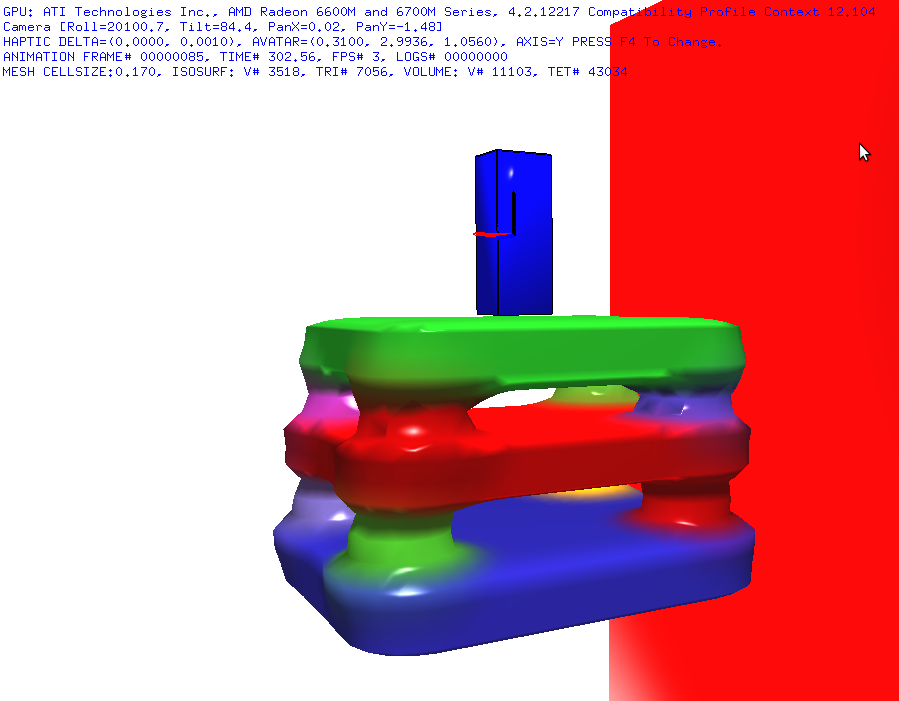
\includegraphics[width=0.30\linewidth]{figures/deformable/shots/cake01.png}
  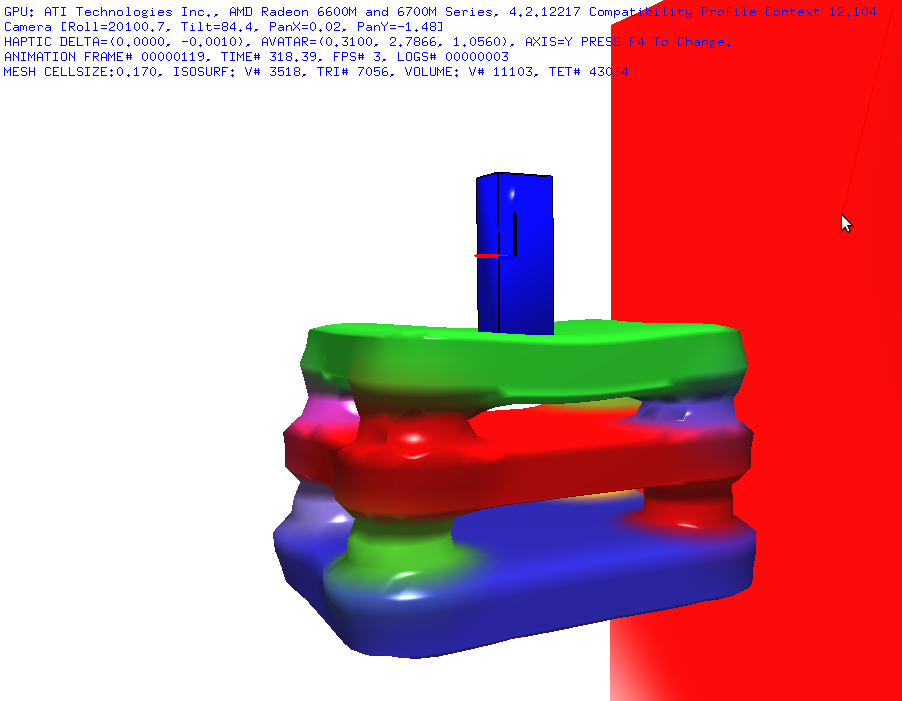
\includegraphics[width=0.30\linewidth]{figures/deformable/shots/cake02.png}
  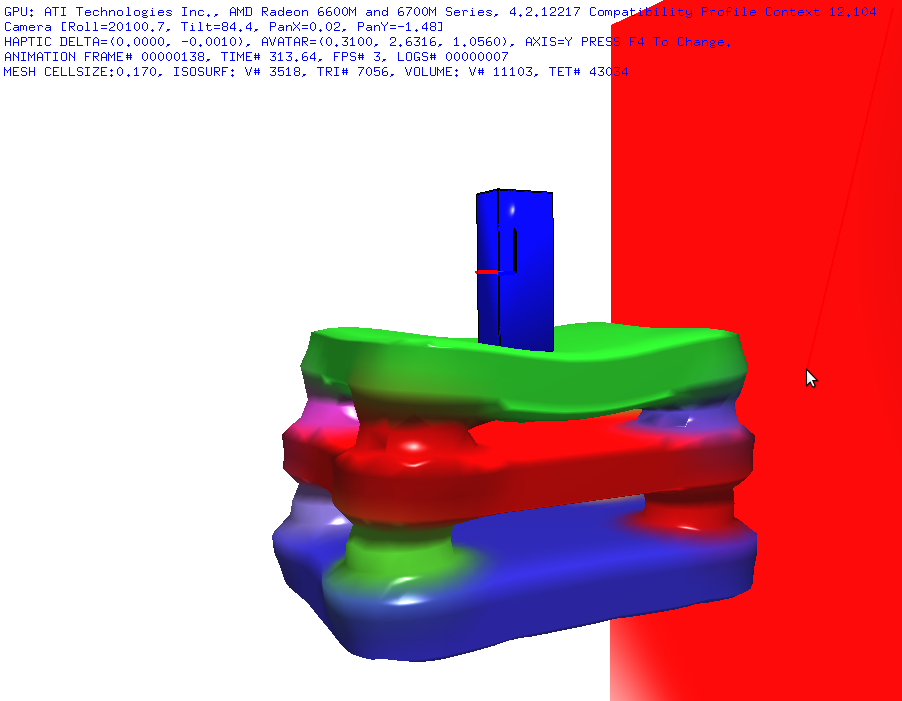
\includegraphics[width=0.30\linewidth]{figures/deformable/shots/cake03.png}

  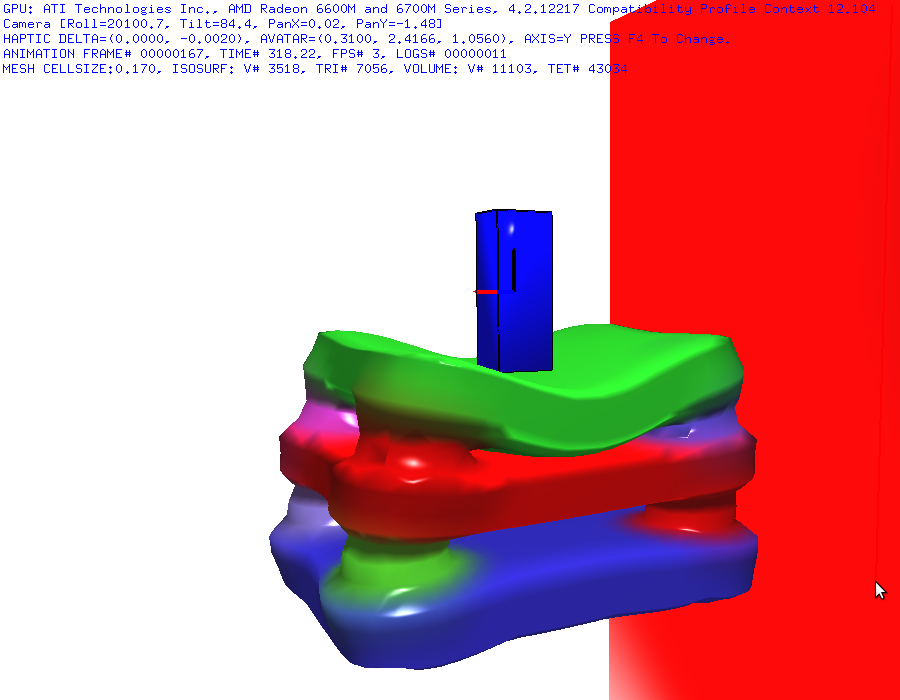
\includegraphics[width=0.30\linewidth]{figures/deformable/shots/cake04.png}
  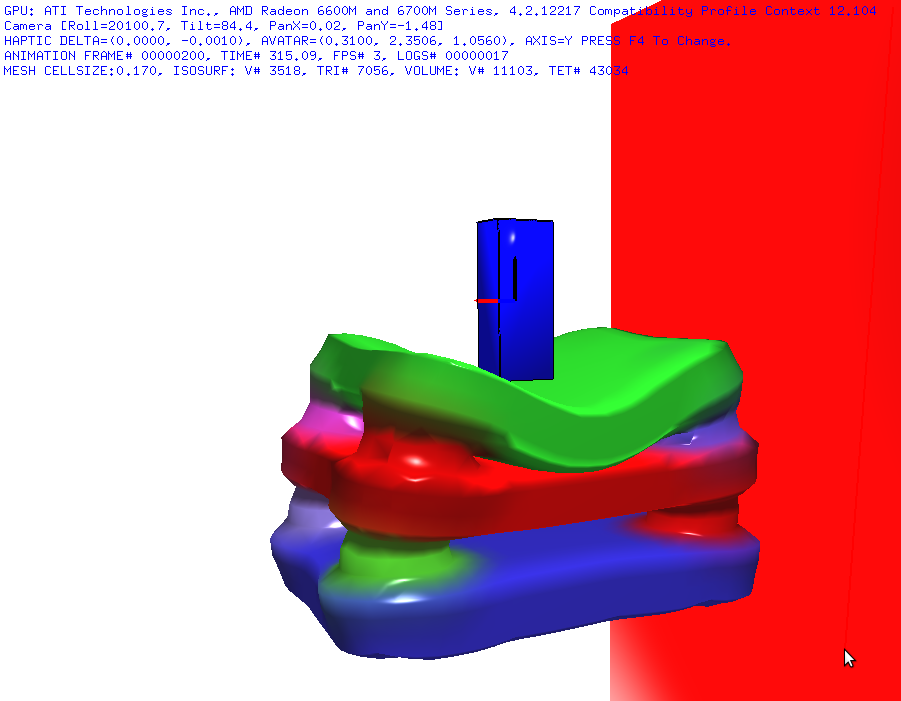
\includegraphics[width=0.30\linewidth]{figures/deformable/shots/cake05.png}
  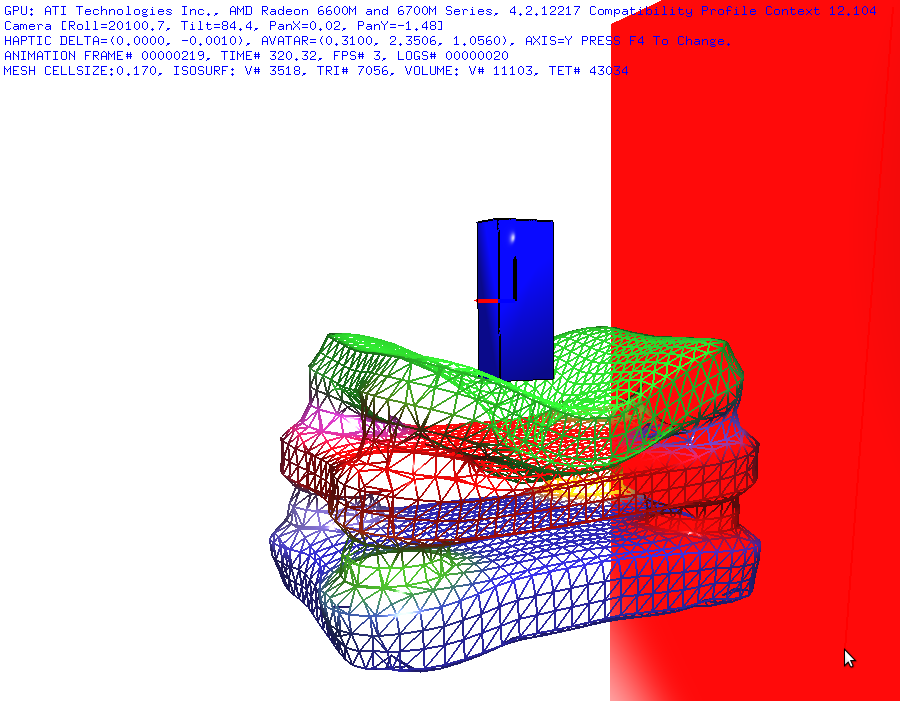
\includegraphics[width=0.30\linewidth]{figures/deformable/shots/cake06.png}

 
  \caption{\label{fig:cake}
  {The cake model is a 3 level structure which is compressed from above in this experiment. The sequence 
  of images show the increasing stages of deformation from the beginning to the end. Last image on the bottom
  row is the surface mesh which is always in sync with the physics model.}
}
\end{figure}

Figure \ref{fig:1ring} shows the contact surface of the probe tool and the volume mesh. The external 
forces are propagated to the volume mesh via the green vertices in the figure. 
All collisions are detected correctly using the technique described in section 
\ref{sec:collisionsandcontacts}.

\begin{figure}[H]
  \centering
  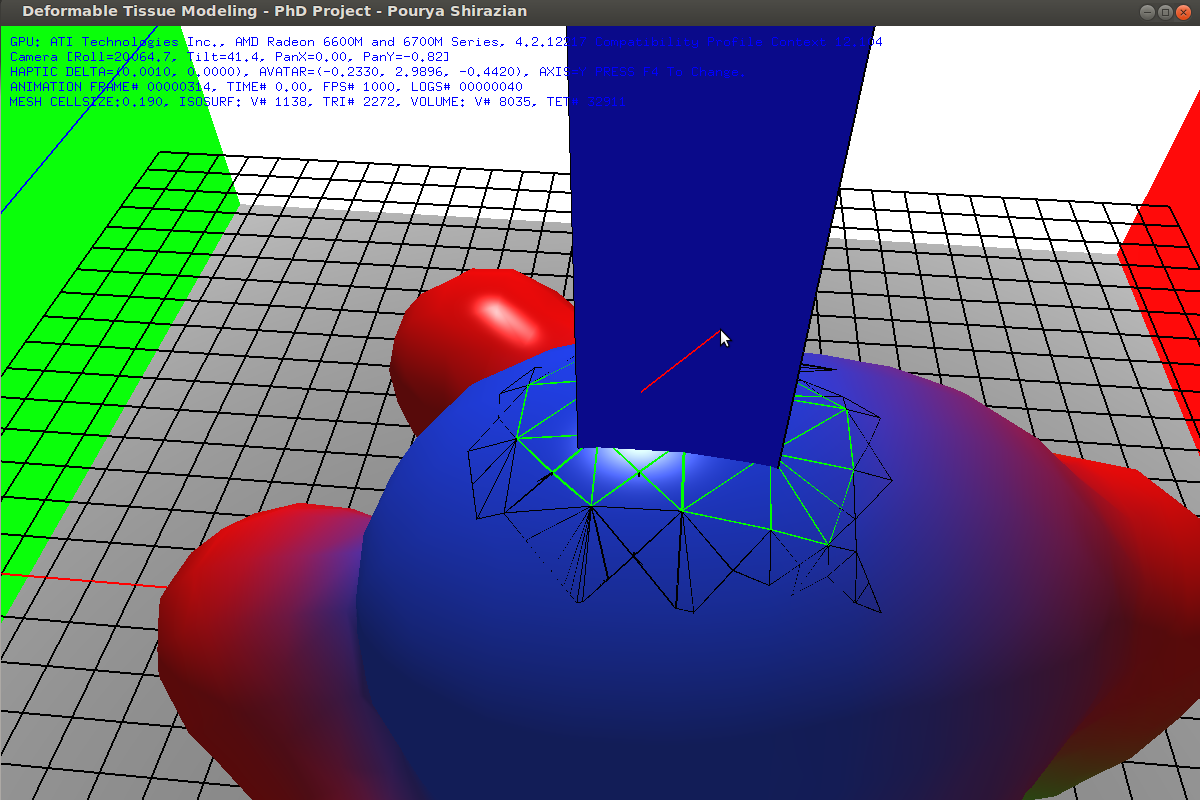
\includegraphics[width=0.45\linewidth]{figures/deformable/shots/1ring01.png}
  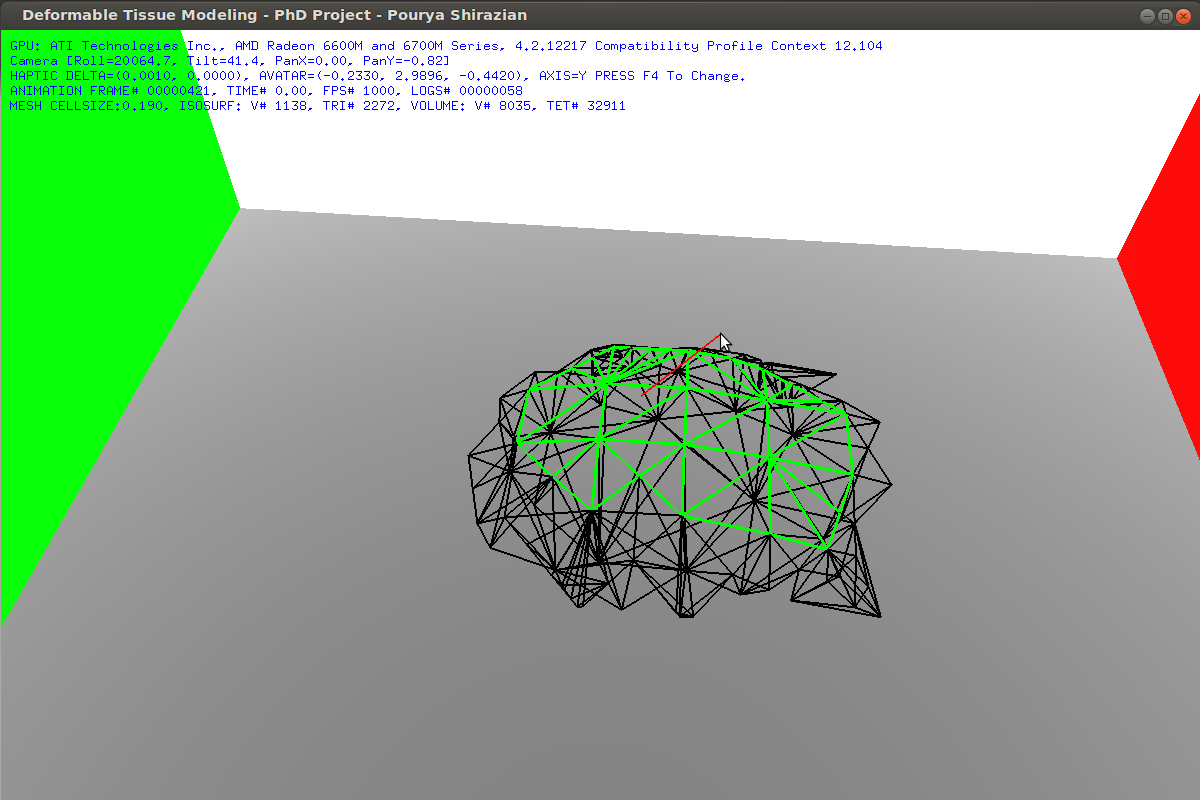
\includegraphics[width=0.45\linewidth]{figures/deformable/shots/1ring03.png}
 
  \caption{\label{fig:1ring}
  {The contact surface of our probe tool and the tumor model shown in green triangles. The computed 
  contact force is applied to all vertices in the green area.}
}
\end{figure}

%

\begin{figure}[H]
  \centering
  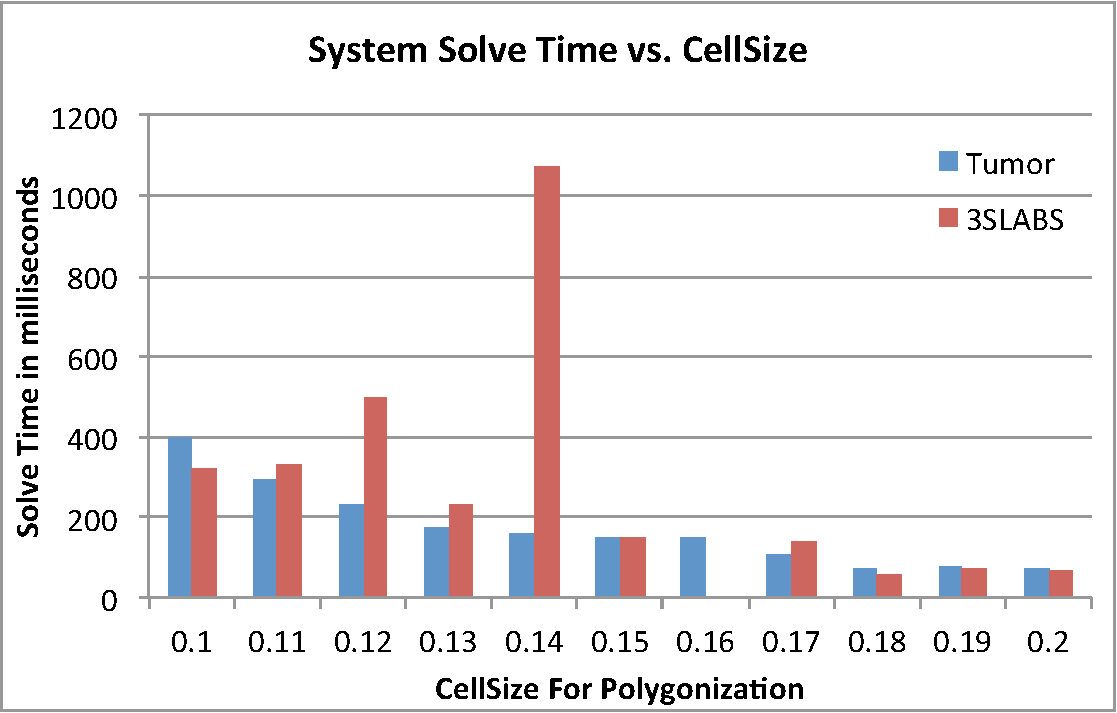
\includegraphics[width=0.8\linewidth]{figures/deformable/systemsolvetime.pdf}
 
  \caption{\label{fig:syssolvetime}
  {System solve time reported in milliseconds vs. the cellsize parameter used for the volume discretization.}
}
\end{figure}

Figure \ref{fig:syssolvetime}, illustrates the system solve time as the cellsize parameter increases 
uniformly. Larger cellsize results in smaller amount of finite element cells which takes less time to solve
for displacements. One way to keep the number of internal tetrahedral cells low 
is by using the adaptive volume discretization technique that uses a coarser grid to extract the elements. 
As overshoot in figure \ref{fig:syssolvetime} at cellsize 0.12 is due to a 
sudden increase in the number of finite element cells despite using a coarser 
grid size. At this point the algorithm was unable to use the coarser grid for 
the internal sampling and a higher percentage of elements are created using the finer grid. 

\begin{figure}[H]
  \centering
  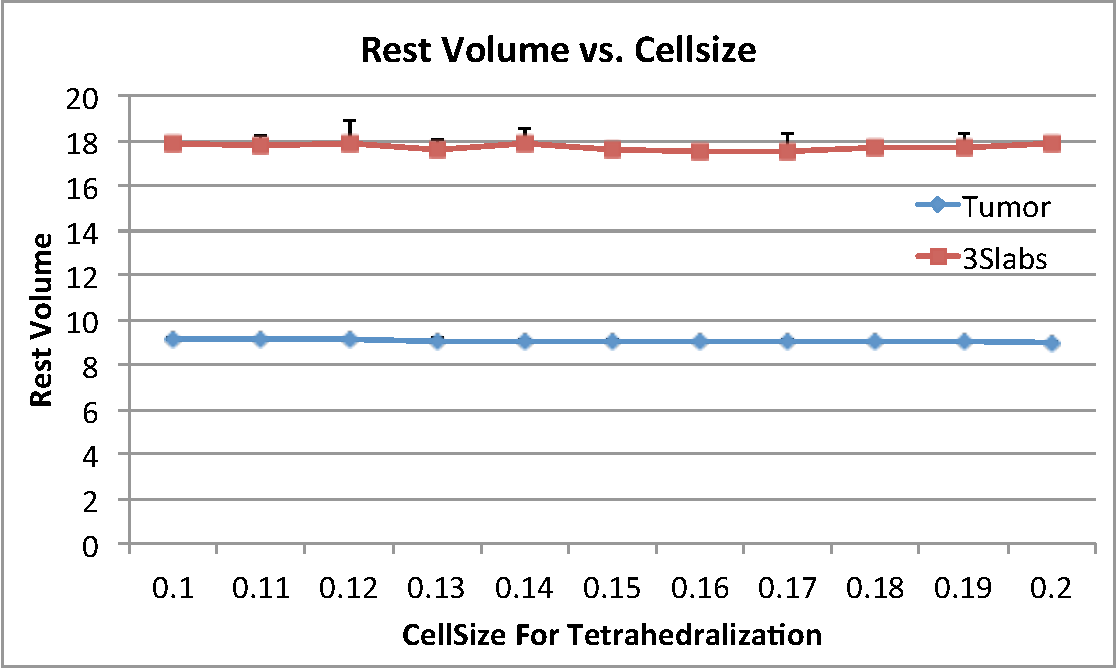
\includegraphics[width=0.8\linewidth]{figures/deformable/volumevscellsize.pdf}
 
  \caption{\label{fig:volumevscellsize}
  {Total volume versus the cellsize parameter for discretization. 
  Maximum volume change in all of our experiments was less than 1 percent.}
}
\end{figure}

One of the required features of a model for surgical simulation scenarios is 
volume preservation. The total volume of the model should not change when it goes under deformations. 

In an experiment, the volume is computed and logged while the model is deformed using the probe tool 
(see figure \ref{fig:volumevscellsize}). Maximum volume change is always less then 1 percent in this test 
for both models and the same results holds under various cellsizes. Both models 
used a constant Poisson ratio of 0.45 in all tests. 















